\section{The Lively Kernel} \label{sec:CONTEXT}

The Lively Kernel is a browser-based runtime and development platform for Web applications, including dynamic graphics, network access, language extensions, object serialization, and development tools. 
Its distinguishing characteristics result from a self-supporting integration of design-time and runtime with sufficient development tools, the implementation of the Morphic User Interface Construction Environment \cite{Maloney1995Mor}, and a serialization mechanism to store objects persistently.

The Lively Kernel itself and some applications are based on the supplied module system that incorporates container modules with namespaces, classes with single inheritance, traits and context-oriented layers \cite{Lincke2011OIC}.
While the integration of development tools into the runtime of the system already shortens the feedback cycle when modyfing such modules \cite{Lincke2012SCS}, Lively further enables developers to compose and script applications with concrete objects only as first promoted by the Self programming language \cite{Ungar1987SPS}:

First, the Morphic architecture allows to directly manipulate and compose new applications out of active components, \emph{Morphs}.
It provides handles for basic graphic modification as resizing, repositioning, and rotating such Morphs, but also ways to add Morphs as children to another Morph.
Second, object-specific behavior provides a concrete context when working on abstract code, allowing developers to try out changes to objects with immediate feedback.
Lively incorporates an Object Editor, shown in \autoref{fig:editor}, that shows all scripts specific to a certain object, allows to add and alter such scripts, and enables developers to experiment with such scripts as all statements without temporary state can be tried for the editor's target object.
Finally, object serialization enables a Web-based object repository \cite{Lincke2012LPC}, called \emph{Parts Bin}, into which developers publish their Morphic creations, called \emph{Parts}. 
Such published parts in the shared repository are available for other Morphic creations, rendering the Parts Bin into a library of visual components that developers can use and reuse.

\begin{figure}
  \centering
  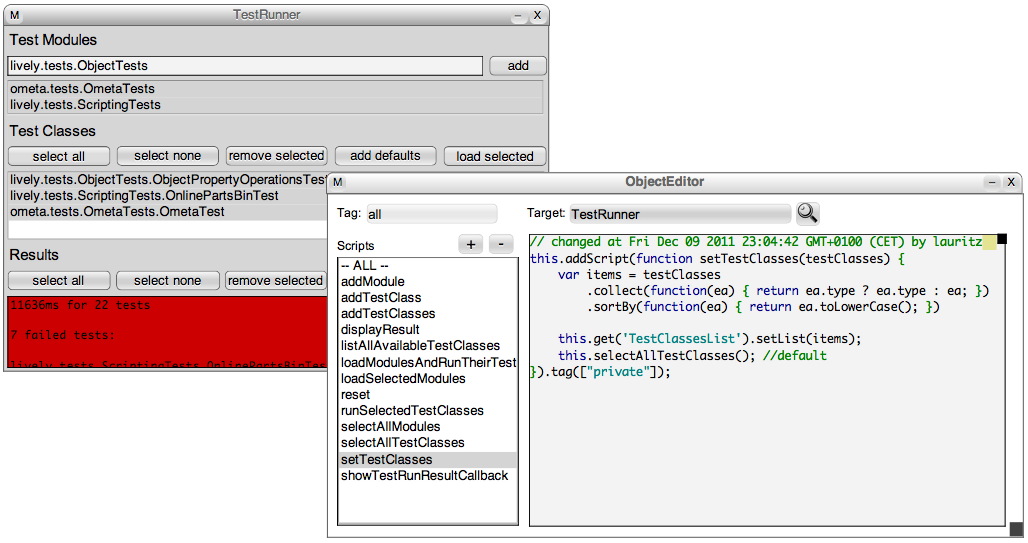
\includegraphics[width=\textwidth]{images/editor}
  \caption{Lively's Object Editor opened on a Test Runner built from Parts.}
  \label{fig:editor}
\end{figure}

This object-centric approach to the creation of applications allows a direct and concrete programming experience in that development happens in the context of a live object that responds to changes immediately.

%%% Local Variables: 
%%% mode: latex
%%% TeX-master: "../paper"
%%% End: 
